\documentclass{article}
\usepackage{pgfornament}
\begin{document}
\definecolor{Maroon}{rgb}{.69,.19,.376}
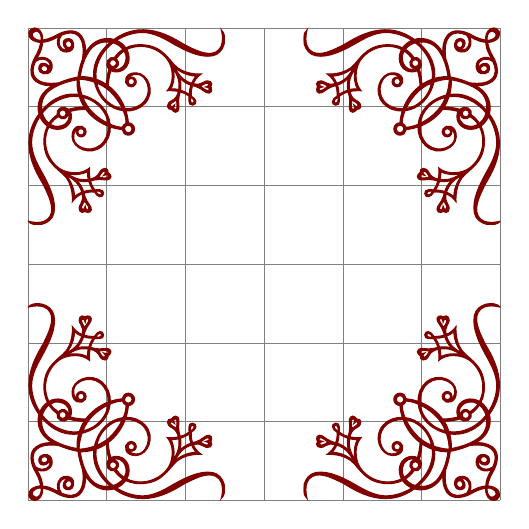
\begin{tikzpicture}[color=Maroon,
                    every node/.style={inner sep=0pt}]
\draw[help lines] (-3,-3) grid (3,3);
\node[minimum size=6cm](vecbox){};
\node[anchor=north west] at (vecbox.north west)
    {\pgfornament[width=2.5cm]{61}};
\node[anchor=north east] at (vecbox.north east)
    {\pgfornament[width=2.5cm,symmetry=v]{61}};
\node[anchor=south west] at (vecbox.south west)
    {\pgfornament[width=2.5cm,symmetry=h]{61}};
\node[anchor=south east] at (vecbox.south east)
    {\pgfornament[width=2.5cm,symmetry=c]{61}};
\end{tikzpicture}
% 图纹
\end{document}
